\section{Multi-Layer Perceptron Classifier}
	    \pagestyle{mario}
	    \sectionauthor{M. Gini \& T. M. Hayden} %\printinunitsof{cm}\prntlen{\linewidth} this shows linewidth in cm

This section presents the multi-layer perceptron (MLP) classifier designed to classify the CIFAR-10 dataset. It is organized as follows: Section \ref{subsec:setup} introduces the basic software setup used to implement the MLP classifier. Section \ref{subsec:preProp} discusses the data preprocessing and augmentation. Section \ref{subsec:netStruct} analyzes the effect of different network structures on performance. Section \ref{subsec:optNet} analyzes what effect varying further hyperparameters like the error function or training algorithm have on the classification performance.

\subsection{Basic Software Setup}\label{subsec:setup}

The neural network toolbox from MATLAB is used to implement the MLP classifier.

\textcolor{red}{maybe picture of basic MLP network}
Since this is a classification problem, parts of the network structure are fixed. The last layer consists of 10 nodes and a in a "softmax" configuration. PICTURE of basic structure.

As a default setup to analzye the effects of parameter variations, the following settings are used:

-stochastic gradient descent training method\\
-cross entropy error function\\
-etc etc\\

\subsection{Data Preprocessing and Augmentation}\label{subsec:preProp}
This subsection discusses the data preprocessing and augmentation.

a) on the selection of the inputs and outputs of the MLP
b) on the size of the training data

\begin{itemize}
   	\item Data Preprocessing

  	The input data is to the network consists of a 3072*1 array where the entries represent the raw pixel values. The pixel values are in the range [0,255]. To avoid any numerical issues and normalize the data, the data is divided by 255 to lie within the range [0,1]. Accordingly, the datatype is changed from the integer format to double. In a second step, the mean per pixel over the whole training set is subtracted. This centers the data.

  	Optionally, we conduct experiments with whitened data. \textcolor{red}{here some plot to show effect of whitened data}

  	\begin{figure}[h!]
  		\centering
  		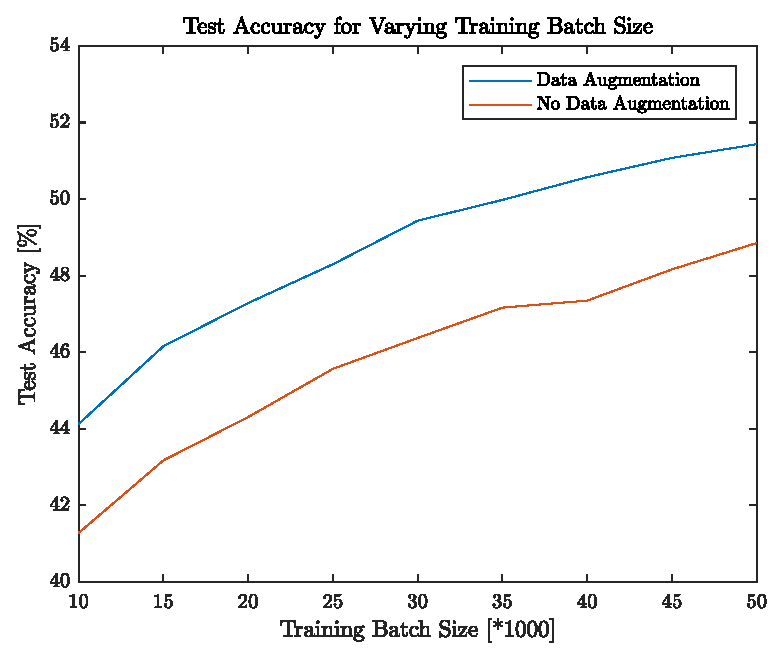
\includegraphics{images/dataAugmentation}
  		\caption{Hello Boy}
  		\label{fig:test1}
  	\end{figure}



  	Data preprocessing also includes the division of the complete dataset into appropriate training, validation and test data batches. The CIFAR-10 dataset consists of 60000 images, with 10000 specifically labeled for testing. For our performance analysis, we always use the provided test batch. The effect of varying training batch size can be seen below \textcolor{red}{here some plot of varying training size}

   	\item Data augmentation

   	Experience shows that a larger training data set increases network performance. A basic and still successful data augmentation method is vertical mirroring. \textcolor{red}{here some plot of varying training size with mirrored data} When comparing with above, the increase in performance can clearly be seen.

\end{itemize}

\subsection{Optimization of Network Structure}\label{subsec:netStruct}

Choosing the correct architecture of a neural network remains a complicated area of study which is still not fully understood\cite{andersen1999cross}. For any given problem there are essentially an infinite number of valid MLP architectures. There are many different approaches to architecture selection but none are foolproof\cite{andersen1999cross}.

\subsubsection{Layers of the MLP}

Every neural network, including MLPs, will have at the very least one input layer and one output layer. The size of the input layer simply depends on the size of the input data. In the case of CIFAR-10 the input size is $32\times32\times3$, the size of the input image data.

In addition to the input layer, each network will also have an output layer. The size of the output layer is also defined by the format of the data. In the the case of CIFAR-10, the output layer is a softmax layer with 10 nodes corresponding to each class label.

There can be an arbitrarily large number of hidden layers. However performance gains from addition additional layers beyond the first are very small or even negligible. Additionally adding more layers increases the chance that the classifier finds a local minima\cite{de1993backpropagation}. Figure \ref{fig:layers} shows the effect of adding additional layers to our MLP classifier. Note that adding additional layers after the 2nd has almost no impact on the test accuracy.

\begin{figure}[h!]
    \centering
    \includegraphics{images/numberlayers}
    \caption{Effect of adding additional layers to the MLP classifier}
    \label{fig:layers}
 \end{figure}


c)on the training of the MLP
\begin{itemize}
   	\item Varying the number of neurons
	\item Varying the number of layers
\end{itemize}

\subsection{Optimization of Network Hyperparameters}\label{subsec:optNet}
Hyperparameter selection for neural networks such as MLPs has become an interesting field of research with many interesting algorithms being used to estimate good parameters to use\cite{bergstra2011algorithms}. However, since these algorithms rely on performing many trials and updating the parameters accordingly, they proved unsuitable for our purposes due to our limited resources. Our approach instead relied on performing a limited number of trails to find trends. From these general trends and our knowledge of MLP classifiers, we then estimated good parameters to use.


d) on the performance of the MLP with different objective functions and optimization methods
\begin{itemize}
   	\item Different learning rates

   	\item Different optimization methods
\end{itemize}
e)any other interesting observation that you think are pertinent (e.g. effect of learning rate on convergence speed).

\subsubsection{Learning Rate}

Choosing the learning rate for a MLP classifier can be a challenging process. There is no approach that will work optimally for every dataset. A learning rate that is too high can overshoot the solution and become unstable. However low learning rates can become stuck in local minima or take a long time to train. A good solution is to pick a high learning rate that can pass over local minima and  to gradually decrease the learning rate so that the classifier does not become unstable. This will result in a classifier which initially follows general trends and 'explores' a large portion of the parameter space. Later on the smaller learning rate will allow for the model to be fine tuned into a particular solution.

The effects of changing the learning rate in our model can be seen in figure \ref{fig:learningRate}. The figure shows that increased learning rates, in general, had a positive effect on model accuracy.


\begin{figure}[h!]
    \centering
    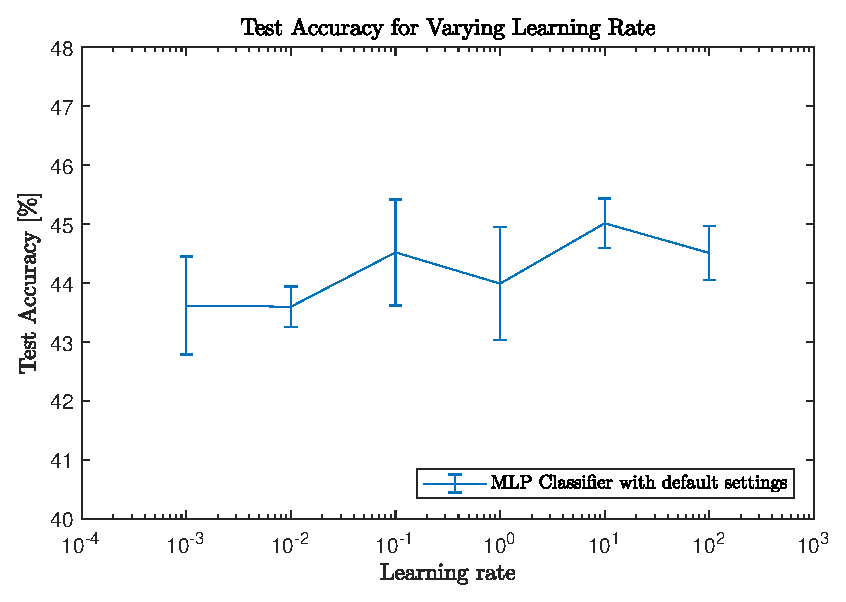
\includegraphics{images/learningRate.eps}
    \caption{2+2=}
    \label{fig:learningRate}
 \end{figure}

 \subsubsection{Performance function}

 \subsubsection{Activation function}

 \subsubsection{Training fucntion}
